% OpenCaseLaw — Paper 2 (flagship, short): the human judicial baseline for
% citation errors, proven against a closed-world reporter series.
% Redrafted 2026-08-13. EVERY scan-derived number regenerates via
% tables/build_tables.py from data/p2_backscan.json (+ p2_probe.json);
% none is transcribed. The remediation facts (letters, replies) are frozen
% from the 2026-08 correspondence (mailbox refs in tables/ REMEDIATION
% comment below) and are the only hand-set numbers.
\documentclass[11pt,a4paper]{article}

\usepackage[T1]{fontenc}
\usepackage{lmodern}
\usepackage{textcomp}
\usepackage[margin=2.5cm]{geometry}
\usepackage[expansion=false,protrusion=false]{microtype}
\usepackage{xcolor}
\usepackage{xurl}
\usepackage[numbers,sort&compress]{natbib}
\usepackage[hidelinks,breaklinks=true]{hyperref}
\emergencystretch=2em
\usepackage{booktabs}
\usepackage{array}
\usepackage{amsmath}
\usepackage{tikz}
\usepackage{float}
\usepackage{authblk}
\newcolumntype{L}[1]{>{\raggedright\arraybackslash}p{#1}}

% ── every scan-derived number: generated, never typed ──
% Auto-generated by tables/build_tables.py — do not edit.
% Source: data/p2_backscan.json (generated 2026-08-13T22:08:33.386943+00:00, graph 2026-08-13T15:18:13.396765+00:00)
\newcommand{\ScanSince}{2024-01-01}
\newcommand{\ScanDate}{2026-08-13}
\newcommand{\ScanGraphDate}{2026-08-13}
\newcommand{\NWindowDecisions}{119{,}214}
\newcommand{\NDenomTokens}{584{,}524}
\newcommand{\NFindings}{591}
\newcommand{\RatePpm}{1{,}011 per million (one in 989)}
\newcommand{\RatePpmBare}{1{,}011}
\newcommand{\RateWilson}{933--1{,}096}
\newcommand{\RateCluster}{931--1{,}093}
\newcommand{\NDecTok}{87{,}063}
\newcommand{\NDecFind}{587}
\newcommand{\DecShare}{0.67\,\%}
\newcommand{\NDistinctRefs}{16{,}708}
\newcommand{\NDistinctTokens}{292}
\newcommand{\DistinctShare}{1.75\,\%}
\newcommand{\NFindingsDe}{210}
\newcommand{\RateDe}{915}
\newcommand{\NFindingsFr}{356}
\newcommand{\RateFr}{1{,}081}
\newcommand{\NFindingsIt}{25}
\newcommand{\RateIt}{970}
\newcommand{\NQuoteMarker}{49}
\newcommand{\QuoteShare}{8.3\,\%}
\newcommand{\NPoolPre}{1{,}646}
\newcommand{\PoolPpm}{2{,}816}
\newcommand{\NPoolPlausible}{278}
\newcommand{\NPoolStart}{21}
\newcommand{\NBareFindings}{1}
\newcommand{\NRawFindings}{1{,}188}
\newcommand{\NDroppedGuard}{596}
\newcommand{\NMechDivision}{272}
\newcommand{\NMechVolume}{103}
\newcommand{\NMechYear}{67}
\newcommand{\NMechDropped}{30}
\newcommand{\NMechPageDigit}{107}
\newcommand{\NMechUnlabelled}{12}
\newcommand{\NRepeatTokens}{89}
\newcommand{\NRepeatFindings}{388}
\newcommand{\TopToken}{BGE 142 I 455}
\newcommand{\TopTokenN}{28}
\newcommand{\SensDedupRate}{500}
\newcommand{\SensQuoteRate}{927}
\newcommand{\NProbeTokens}{292}
\newcommand{\NProbeConfirmed}{254}
\newcommand{\NProbeExists}{0}
\newcommand{\NProbeOOC}{38}
\newcommand{\NProbeCand}{115}
\newcommand{\NProbeCandExist}{109}
\newcommand{\NFindConfirmed}{542}
\newcommand{\NFindOOC}{49}
\newcommand{\NMechMulti}{464}
\newcommand{\NMechSingle}{115}
\newcommand{\NMechNone}{12}
\newcommand{\RateFederal}{877}
\newcommand{\RateCantonal}{1{,}064}
\newcommand{\NFederalFindings}{147}
\newcommand{\PFedCant}{0.04}
\newcommand{\ChiLang}{3.8}
\newcommand{\SensDedupRateDistinct}{17{,}477}


% ── FROZEN remediation facts, 2026-08 correspondence ──
% Source: outgoing letters of 2026-08-03 and court replies of
% 2026-08-04..06 (author's mail archive, refs 1449..1611, 1649).
% Verified fact: seven court administrations replied within three
% days. Courts are deliberately not named anywhere in this paper
% (author decision 2026-08-13); the letter/addressee count is not
% independently enumerated and the paper does not state one.
\newcommand{\RLetterDate}{3 August 2026}
\newcommand{\RNReplied}{seven}
\newcommand{\RNReplyDays}{three}

\title{When Courts Miscite: A Provable Baseline for Citation Errors\\
in Swiss Judicial Decisions}

\author[1]{Jonas Hertner}
% Provisional CRediT (add on confirmed acceptance of co-authorship):
% Merane methodology/validation/legal analysis/writing; Zollikofer
% software/formal analysis/reproducibility; Ash methodology/supervision/
% formal analysis/writing; Hertner conceptualisation/data curation/
% software/investigation/resources/writing.
\affil[1]{OpenCaseLaw}

\begin{document}
\maketitle

\begin{abstract}
Measurement studies report legal hallucination in 58--88\,\% of
responses to case-law queries put to large language
models~\cite{dahl2024} and in 17--33\,\% for commercial legal-RAG
tools~\cite{magesh2024}. These figures lack a reference point: how
often do \emph{courts themselves} cite authority that does not exist?
We give, to our knowledge, the first decidability-based answer for a
national jurisdiction. The Swiss Federal Supreme Court's official
reporter (BGE/ATF/DTF) is a closed, continuously paginated series,
held completely in our corpus from 1875; the nonexistence of a cited
locus is therefore decidable. Scanning \NDenomTokens{} distinct
reporter-citation edges (one per decision and cited locus) in
\NWindowDecisions{} Swiss decisions issued since January 2024, we find
\NFindings{} provably nonexistent citations --- \RatePpm{}, Wilson
95\,\% \RateWilson{} ppm, decision-cluster bootstrap \RateCluster{}
ppm. The machine studies measure responses and count existent-but-wrong
citations; we measure citations and count provable nonexistence only.
The units are not divisible into a ratio, so we state them side by
side: roughly one citation in a thousand in the published human record,
against 17--88\,\% of machine responses under broader error
definitions. The court's public resolver independently confirms the
scan --- \NFindConfirmed{} of \NFindings{} findings carry a token the
resolver 404s, none resolves --- and because the series is closed,
most errors carry a local-damage signature: for \NMechDivision{}
findings the cited page exists under a sibling division of the same
volume, and where the citing document itself states the intended
citation, the deterministic repair reproduces it exactly. Errors
concentrate in reused boilerplate --- one mistyped division letter
recurs verbatim in three decisions across two court levels. Reported
to the issuing courts on \RLetterDate{}, the findings drew replies
from \RNReplied{} court administrations within \RNReplyDays{} days;
two courts confirmed corrections, one already implemented. A record
that can be audited can be healed. Every scan-derived number
regenerates from released, hash-manifested artifacts.
\end{abstract}

%==================================================================
\section{Introduction}\label{sec:intro}

The reliability of legal citations has become a measured quantity.
\citet{dahl2024} report hallucination in 58--88\,\% of responses to
reference-based case-law queries put to general-purpose LLMs;
\citet{magesh2024} measure 17--33\,\% for commercial legal-RAG
products; a public registry
documents over 1{,}300 court proceedings in which judges confronted
AI-generated citations in filings~\cite{charlotin2026}. Detection work
has followed: verification against a national citation
graph~\citep{ovcharov2026ukraine}, benchmarks with injected
hallucinations~\citep{legalcitebench2026}, and surveys of detection
tools~\citep{citetools2026}. Verifying citations is now framed as a
burden courts themselves need help with~\citep{citp2026}.

Every one of these numbers floats without a baseline. Fabrication rates
are alarming relative to an implicit assumption --- that human legal
writing cites what exists --- which no study quantifies. The nearest
observation is an aside: a hallucination-detection benchmark built on
pre-LLM briefs notes ``over 10 human-made citation typos'' in its
source material and moves on~\citep{legalcitebench2026}. Measuring the
human side properly requires something unusual: a corpus in which the
\emph{nonexistence} of a cited authority is provable rather than merely
unresolved. Reference-error studies in other fields illustrate the
difficulty: quotation-error rates near 20\,\% are reported in medical
literature~\citep{quotationerr}, but against open-ended reference
universes where absence of evidence remains evidence of nothing.

Swiss law provides the unusual conditions. The Federal Supreme Court's
official reporter --- \emph{BGE} in German, \emph{ATF} in French,
\emph{DTF} in Italian; one series, three prefixes --- is closed and
continuously paginated: volume and division fix a page range, decisions
begin at known pages, and the series is complete in our corpus from
1875 to the present~\citep{hertner2026opencaselaw}. For a citation of
the form \emph{BGE 148 I 356}, existence is therefore decidable: either
some reported decision begins at (or plausibly contains) that locus, or
none does. ``Provably nonexistent'' is a statement about a finite,
enumerable set, not a retrieval failure.

We scan the reporter citations of every Swiss decision issued since
January 2024 in the corpus --- \NDenomTokens{} distinct citation edges
(the extractor counts each cited locus once per decision) across
\NWindowDecisions{} decisions from federal and cantonal courts in all
three official languages --- and prove nonexistence for \NFindings{}:
\RatePpm{}. The baseline the field has been missing can then be stated
next to the machine numbers, each in its own unit: roughly 0.1\,\% of
citations in the published human record, against 17--33\,\% of
commercial legal-RAG responses and 58--88\,\% of raw-LLM responses
under broader error definitions --- the differences in unit, universe
and definition are laid out in Table~\ref{tab:comparability} rather
than divided away.

Three further contributions come from reading the errors rather than
counting them. First, a \textbf{mechanism taxonomy}, computed
deterministically over every finding rather than curated from examples:
human miscitation overwhelmingly matches local-damage signatures of a
true citation --- a division letter substituted while the page stays
right, a digit doubled or dropped, a year where a page belongs ---
where LLM fabrication invents whole plausible loci. In \NMechDivision{} of
\NFindings{} findings the cited page exists as a decision start under a
\emph{sibling division of the same volume}. Second,
\textbf{propagation}: identical erroneous tokens recur across decisions,
courts and years, carried by reused doctrinal passages --- the token
\emph{BGE 147 IIII 249}, division III with a doubled letter, appears
verbatim in three decisions across two court levels, each quoting the
same standard. Third, a \textbf{remediation loop with observed
outcomes}: the findings were verified, reported to the issuing courts
on \RLetterDate{}, and drew replies from \RNReplied{} court
administrations within \RNReplyDays{} days, including two confirmed
corrections (Section~\ref{sec:campaign}). A record that can be audited can also be
healed.

\paragraph{What this paper is not.} It does not rank courts, and it
does not claim the found errors affected outcomes: a wrong volume
number beside a correct parallel citation is a blemish, not a
miscarriage. The rate we report is a property of the published record,
offered as the denominator the machine-fabrication literature lacks.

%==================================================================
\section{Related work}\label{sec:related}

\paragraph{LLM citation fabrication.} \citet{dahl2024} established
hallucination rates for general-purpose models over fourteen tasks on
the U.S.\ federal judiciary --- nine reference-based, five
reference-free; their pooled 58--88\,\% covers the reference-based
tasks, which span existence, court, citation, author, disposition and
more; \citet{magesh2024} extended measurement to commercial legal-RAG
tools with 202 preregistered queries; \citet{charlotin2026} tracks
court-confronted instances. Detection approaches verify model output
against citation graphs~\citep{ovcharov2026ukraine}, benchmark
detectors on synthetic corruptions~\citep{legalcitebench2026}, or
survey tool capabilities~\citep{citetools2026}. All measure or police
the machine side; none that we found measures the human side, which is
this paper's object.\footnote{Sweep documented in the released
\texttt{notes/novelty-audit.md}: the LLM-hallucination literature and
its surveys, legal citation-infrastructure studies, and
reference-error studies in scientific writing. Bluebook-error,
citator-accuracy and non-English empirical literatures are searched
but not exhaustively; the claim is scoped ``to our knowledge''
accordingly.}

\paragraph{Reference errors in human writing.} Citation and quotation
error rates are long studied in scientific
literature~\citep{quotationerr}, with majorities of surveyed articles
containing at least minor reference defects. Those studies rely on
manual lookup in open-ended bibliographic universes; the closed-world
reporter series lets us replace sampling with exhaustive scanning and
judgment with decidability, at the price of covering only
reporter-form citations. For judicial opinions specifically, the
nearest empirical work measures \emph{link rot}: 29\,\% of internet
links cited in U.S.\ Supreme Court opinions 1996--2010 no longer
worked~\citep{liebler2013}. Rot is post-publication decay of the
referent; our object is publication-time nonexistence of the cited
authority.

\paragraph{Swiss legal data.} The corpus and citation graph underlying
this study are described in the companion resource
paper~\citep{hertner2026opencaselaw}; the Swiss Federal Supreme Court
Dataset~\citep{geering2024scd} provides structured metadata for the
federal layer.

%==================================================================
\section{Method}\label{sec:method}

\subsection{Decidability conditions}\label{sec:decidable}

A reporter citation names a volume $v$, a division $d$, and a page $p$.
The series is continuously paginated within each (volume, division):
decisions begin at strictly increasing pages, and a decision occupies
the pages from its start to the next decision's start. Our corpus holds
every reported decision since volume~1 (1875), giving for each $(v,d)$
the complete sorted list of start pages $S_{v,d}$
(Figure~\ref{fig:decidability}).

A cited locus $(v,d,p)$ is \textbf{provably nonexistent} iff one of:
\begin{enumerate}
\item \emph{Division absent}: $S_{v,d} = \emptyset$ although volume $v$
      exists (the reporter's divisions are I, Ia, Ib, II, III, IV, V;
      the Ia/Ib split existed 1955--1994 and is evaluated as a family
      with I, since citations casefold the sub-letter).
\item \emph{Page beyond the series}: $p > \max S_{v,d} + w_{v,d}$, where
      the window $w_{v,d}$ is the longest observed decision length in
      that $(v,d)$, with a floor of 30 pages --- a mid-volume page can
      always be a legitimate deep pin-cite, so only pages beyond the
      last decision's plausible extent are provable.
\item \emph{Volume out of range}: $v$ exceeds the newest volume by more
      than one (the newest two volumes are still filling and are exempt
      from all three conditions).
\end{enumerate}
Everything else --- including citations that merely fail to resolve ---
is \emph{not} counted, and nonexistence is asserted as of the citing
decision's date (a volume beyond next year's does not exist when cited,
though it may later).

The three conditions differ in epistemic strength. Division-absent and
volume-out-of-range are decidable from the series structure alone.
Page-beyond-the-series depends on the window $w_{v,d}$, which is
inductive --- the final decision of a $(v,d)$ could in principle exceed
every predecessor's length. We therefore close the gap externally: the
court's own resolver redirects any page \emph{inside} a decision to
that decision and returns 404 otherwise (Section~\ref{sec:guards}), so
a 404 is an authoritative statement that no decision contains the
cited page. Of the \NFindings{} findings, \NFindConfirmed{} carry a
token the resolver 404s; the remaining \NFindOOC{} cite volumes below
the resolver's coverage floor and rest on the corpus proof and the
window rule alone.

% Auto-generated by tables/build_tables.py
% Data: bge_series_index.json — BGE 139 II starts (last 534,
% window 48); BGE 148 I last start 295;
% 356 IS a start in 148 IV.
\begin{figure}[t]
\centering
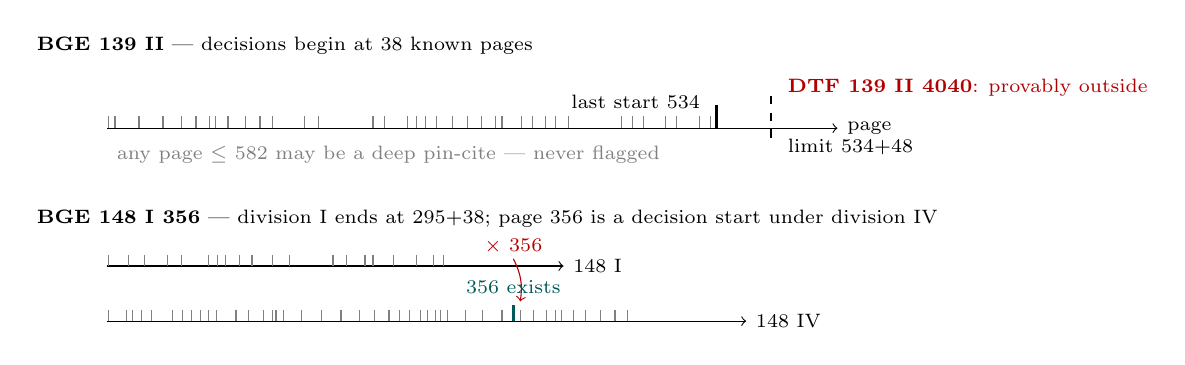
\begin{tikzpicture}[x=0.0145cm, y=1cm, font=\scriptsize]
% ── panel 1: page axis of BGE 139 II ──
\node[anchor=west] at (-70, 1.05) {\textbf{BGE 139 II} ---
  decisions begin at 38 known pages};
\draw[->] (0,0) -- (640,0) node[right] {page};
\foreach \p in {1, 7, 28, 49, 65, 78, 90, 95, 106, 121, 134, 145, 173, 185, 233, 243, 263, 271, 279, 289, 303, 316, 328, 340, 346, 363, 373, 384, 393, 404, 451, 460, 470, 489, 499, 519, 529, 534}
  \draw[gray] (\p, 0) -- (\p, 0.16);
\draw[very thick] (534,0) -- (534,0.3);
\node[anchor=east] at (528, 0.34) {last start 534};
\draw[thick, dashed] (582,-0.12) -- (582,0.46);
\node[anchor=west] at (588, -0.24)
  {limit 534$+$48};
\node[red!70!black, anchor=west] at (588, 0.52)
  {\textbf{DTF 139 II 4040}: provably outside};
\node[anchor=west, gray] at (0, -0.34) {any page $\leq$
  582 may be a deep pin-cite --- never flagged};
% ── panel 2: division absent / substitution ──
\node[anchor=west] at (-70, -1.15) {\textbf{BGE 148 I 356} ---
  division I ends at 295$+$38;
  page 356 is a decision start under division IV};
\draw[->] (0,-1.75) -- (400,-1.75) node[right] {148 I};
\foreach \p in {1, 19, 33, 53, 65, 89, 97, 104, 116, 127, 145, 160, 198, 210, 226, 233, 251, 271, 286, 295}
  \draw[gray] (\p,-1.75) -- (\p,-1.61);
\node[red!70!black] at (356,-1.5) {$\times$ 356};
\draw[->] (0,-2.45) -- (560,-2.45) node[right] {148 IV};
\foreach \p in {1, 17, 22, 30, 39, 57, 66, 74, 82, 89, 96, 113, 124, 137, 145, 148, 155, 170, 188, 205, 221, 234, 247, 256, 265, 275, 281, 288, 292, 298, 314, 329, 346, 356, 362, 374, 385, 393, 398, 409, 419, 432, 445, 456}
  \draw[gray] (\p,-2.45) -- (\p,-2.31);
\draw[very thick, teal!70!black] (356,-2.45) -- (356,-2.24)
  node[above] {356 exists};
\draw[->, red!70!black] (356,-1.66) to[bend left=18] (362,-2.2);
\end{tikzpicture}
\caption{Decidability on the closed series, drawn from the released
index. Top: continuous pagination fixes, for every (volume, division),
the last decision start and an adaptive window; only pages beyond that
limit are flagged. Bottom: \emph{BGE 148 I 356} is provably
nonexistent --- and the same page is a decision start under division IV,
the deterministic \emph{division substitution} signature.}
\label{fig:decidability}
\end{figure}


\subsection{Guards against false positives}\label{sec:guards}

Five mechanisms, each added after a concrete failure it now prevents:
\begin{itemize}
\item \textbf{Own-OCR exclusion.} A corpus-wide scan back to 1875 flags
      $\sim$1{,}500 tokens, concentrated in 19th-century decisions
      where the flagged token is our OCR of the source, not the court's
      text. The study window (since 2024) is born-digital, and every
      finding's context excerpt is carried in the release for
      inspection.
\item \textbf{Prefix discipline for bare tokens.} French and Italian
      typography breaks citations across lines, and older French texts
      write dates with Roman months (\emph{31 III 2004}). The primary
      universe is therefore \emph{prefixed} citations only. A token
      without its own BGE/ATF/DTF prefix is admitted to a separately
      reported secondary channel only if the source text shows the
      prefix immediately before it and the preceding character is not a
      digit (excluding digit-split artefacts like \emph{1 43 V 409});
      this channel contributed \NBareFindings{} finding, excluded from
      every headline number. Of \NRawFindings{} raw flags,
      \NDroppedGuard{} failed these guards and were dropped.
\item \textbf{Pin-cite window.} Continuous pagination makes any
      mid-volume page a possible deep pin-cite; the adaptive window
      $w_{v,d}$ (Section~\ref{sec:decidable}) prevents the class of
      false flags where a long leading case is cited 30+ pages into its
      body.
\item \textbf{Open-volume exemption.} The newest volumes are still
      publishing; nothing in them (or one volume beyond) is decidable
      and nothing is flagged.
\item \textbf{Grammar coverage.} The extractor recognises divisions
      written I--V. Citations using the historical sub-divisions Ia/Ib
      (volumes 81--120, 1955--1994) --- \emph{BGE 120 Ia 45} --- are
      not extracted and enter neither numerator nor denominator: a
      raw-text count puts this class at 10{,}723 occurrences in
      6{,}826 window decisions, 1.4\,\% of the reporter-citation
      surface. The rate is therefore a property of I--V-form
      citations (Section~\ref{sec:limits}).
\item \textbf{External cross-check.} Every distinct flagged token was
      probed against the Federal Supreme Court's public resolver, whose
      semantics we verified directly: a decision start returns its own
      page, an interior page redirects to the containing decision
      (existence proven), a nonexistent locus returns 404. Of
      \NProbeTokens{} distinct tokens, \NProbeOOC{} lie in volumes
      below the resolver's coverage floor (volume 80, 1954; real older
      citations also 404 and rest on the corpus proof). All
      \NProbeConfirmed{} tokens within coverage return 404 and
      \NProbeExists{} resolve --- zero scan false positives on the
      testable set. The resolver also \emph{positively} confirms the
      repair candidates of Section~\ref{sec:taxonomy}:
      \NProbeCandExist{} of \NProbeCand{} unique candidates exist; the
      remainder are themselves below the coverage floor, none is
      refuted.
\end{itemize}

\subsection{Voice}\label{sec:voice}

A court's text sometimes \emph{reports} a party's erroneous citation
rather than committing one. We screen all findings with a deterministic
quotation-marker detector (typographic quotation characters in the
context excerpt): \NQuoteMarker{} of \NFindings{} findings
(\QuoteShare) carry markers. Reading each flagged context, three are
attributed to a party rather than the court: an appellate court flags
the appellant's \emph{BGE 419 III 210} as erroneous and supplies the
correction (the citation enters our graph because the erroneous token
appears verbatim in the decision text); one decision summarises a
debtor's contention in reported speech; one enumerates the
authorities the parties cite while holding that none supports them.
The sensitivity row of Table~\ref{tab:sensitivity} excludes all
\NQuoteMarker{} marker-carrying findings and moves the rate by about
8\,\%. Reported speech without typographic markers remains a residual
risk, stated in Section~\ref{sec:limits}; the reading is a
single-reader pass by the author, not a protocolised multi-annotator
adjudication.

\subsection{Denominator}\label{sec:denominator}

The denominator is counted in the same pass that produces the
findings: every distinct prefixed (decision, locus) edge the classifier
considered --- \NDenomTokens{} edges from \NWindowDecisions{}
decisions, of which \NDecTok{} cite the reporter at least once. The
unit is deliberately the edge, not the mention: the extractor counts a
cited locus once per decision, so a decision repeating the same wrong
citation five times contributes one finding and one denominator entry,
and resolved edges carrying several graph target rows are counted
once. Per-language and per-form denominators, and the per-decision
cluster structure used for the bootstrap, are released with the data.

%==================================================================
\section{Results}\label{sec:results}

\subsection{The rate}\label{sec:rate}

Table~\ref{tab:rates} states the headline three ways. Per citation
edge: \NFindings{} of \NDenomTokens{} distinct prefixed reporter
citations are provably nonexistent, \RatePpm{}. Per decision:
\DecShare{} of the \NDecTok{} decisions that cite the reporter contain
at least one provable error. Per distinct locus: \NDistinctTokens{}
distinct erroneous tokens against \NDistinctRefs{} distinct cited
loci. The window is a census of the corpus, so the intervals are not
sampling corrections for these counts; they quantify uncertainty about
the decision-generating process, reading the window as one draw from
it. Beside the Wilson interval we report a bootstrap that resamples
decisions; the two nearly coincide because the extractor's
edge-per-decision unit already removes within-decision repetition
(\NDecFind{} decisions carry the \NFindings{} findings). Dependence
\emph{across} decisions --- the shared boilerplate of
Section~\ref{sec:propagation} --- is not captured by either interval;
the distinct-locus row is the view least affected by it.

% Auto-generated by tables/build_tables.py
\begin{table}[t]
\centering\small
\caption{Provably nonexistent reporter citations in Swiss decisions
issued since \ScanSince{} (scan of 2026-08-13, graph of 2026-08-13).
Wilson 95\,\% intervals; the headline per-token rate additionally
carries a cluster-bootstrap interval by decision
(10{,}000 replicates).}
\label{tab:rates}
\begin{tabular}{l r r r l}
\toprule
Unit & Errors & Universe & Rate (ppm) & 95\,\% CI (ppm) \\
\midrule
Citation tokens & 591 & 584{,}524 & 1{,}011 &
  933--1{,}096 (cluster 931--1{,}093) \\
Decisions ($\geq$1 finding) & 587 & 87{,}063 &
  6{,}742 & 6{,}220--7{,}308 \\
Distinct cited loci & 292 & 16{,}708 &
  17{,}477 & 15{,}598--19{,}577 \\
\bottomrule
\end{tabular}
\end{table}


Per language (Table~\ref{tab:languages}): German \RateDe{}, French
\RateFr{}, Italian \RateIt{} per million. A homogeneity test does not
detect a difference ($\chi^2{=}\ChiLang$, 2~df) --- absence of
evidence for a difference, not evidence of equality. Across court
classes the data do show a difference: federal decisions run at
\RateFederal{} and cantonal decisions at \RateCantonal{} per million
(nominal two-sided $p{=}\PFedCant$, Table~\ref{tab:sensitivity}); the
federal stratum still contributes \NFederalFindings{} findings in the
federal courts' own published texts.

% Auto-generated by tables/build_tables.py
\begin{table}[t]
\centering\small
\caption{Per-language rates over distinct prefixed citation edges,
with Wilson 95\,\% intervals.}
\label{tab:languages}
\begin{tabular}{l r r r l}
\toprule
Language & Errors & Tokens & Rate (ppm) & Wilson 95\,\% \\
\midrule
German & 210 & 229{,}561 & 915 & 799--1{,}047 \\
French & 356 & 329{,}180 & 1{,}081 & 975--1{,}200 \\
Italian & 25 & 25{,}783 & 970 & 657--1{,}431 \\
\bottomrule
\end{tabular}
\end{table}


% Auto-generated by tables/build_tables.py
% Definitions extracted from the primary sources (novelty-audit.md).
\begin{table*}[t]
\centering\small
\caption{What each study measures. The rates are not directly
comparable --- the units differ --- which is precisely why the human
baseline must be stated in its own unit rather than inferred from the
machine studies.}
\label{tab:comparability}
\begin{tabular}{L{2.6cm} L{3.6cm} L{3.6cm} L{4.6cm}}
\toprule
 & Dahl et al.~2024 & Magesh et al.~2025 & This study \\
\midrule
Unit & response to a case-law query & response to a legal research
query & distinct citation edge in a published decision \\
Population & 4 general LLMs; stratified federal case sample & 3
commercial legal-RAG tools + GPT-4 & every Swiss decision issued since
2024 in the corpus \\
Universe & 14 QA tasks: 9 reference-based, 5 reference-free;
$n{=}5{,}000$ per court level, $n{=}100$ high-complexity & 202
preregistered queries & \NDenomTokens{} prefixed reporter-citation
edges \\
Detection & reference-based: contradiction with known metadata;
reference-free: self-contradiction & human coding of responses and
cited sources & decidable nonexistence against the complete reporter
series, cross-checked on the court's resolver \\
Error definition & response inconsistent with legal facts (existence,
court, citation, author, disposition, \ldots) & false statement, or
source that does not support the claim & cited locus provably absent
from the series \\
Includes wrong-but-existent citations & yes & yes & no (floor) \\
Headline & 58--88\,\% of responses, reference-based tasks pooled by
model & 17--33\,\% of responses (GPT-4 43\,\%) & \RatePpmBare{}
ppm of citations \\
\bottomrule
\end{tabular}
\end{table*}


Table~\ref{tab:comparability} aligns this measurement with the machine
studies. The units differ by construction --- responses to elicitation
there, spontaneous citations in published text here --- and our
definition is strictly narrower: \citet{dahl2024} and
\citet{magesh2024} count wrong-but-existent citations as
hallucinations, which our closed-world method deliberately cannot see.
Excluding the wrong-but-existent class makes our numerator a floor
against a stricter standard; it also means the table's rates answer
different questions, which is why we present them side by side and do
not report a ratio.

\subsection{Mechanism taxonomy}\label{sec:taxonomy}

Because the series is closed, most errors match a local-damage
signature. For every finding we evaluate deterministic rules --- pure
functions of the token and the series index, released with the code
--- in fixed priority order (Table~\ref{tab:mechanisms}). The labels
are signatures, not causal attributions: \NMechMulti{} of \NFindings{}
findings satisfy more than one rule, \NMechSingle{} exactly one,
\NMechNone{} none, and the table counts the first match in priority
order. What the signatures establish is proximity: a small, structured
edit maps the erroneous token onto an existing locus.

% Auto-generated by tables/build_tables.py
\begin{table}[t]
\centering\small
\caption{Deterministic mechanism labels over all \NFindings{}
findings: each label is a pure function of the token and the series
index (Section~\ref{sec:taxonomy}). A finding may satisfy several
rules; the first in priority order is counted.}
\label{tab:mechanisms}
\begin{tabular}{l r r r r}
\toprule
Mechanism & DE & FR & IT & Total \\
\midrule
Division substitution & 92 & 169 & 11 & 272 \\
Volume substitution & 45 & 56 & 2 & 103 \\
Extra digit in page & 28 & 64 & 6 & 98 \\
Year in page position & 20 & 43 & 4 & 67 \\
Dropped leading volume digit & 16 & 14 & 0 & 30 \\
Unlabelled residual & 5 & 6 & 1 & 12 \\
Doubled digit in page & 4 & 4 & 1 & 9 \\
\bottomrule
\end{tabular}
\end{table}


\begin{itemize}
\item \textbf{Division substitution} (\NMechDivision{} findings, the
      dominant class): the cited page exists as a decision start under
      a sibling division of the same volume. Two criminal-division
      decisions print \emph{BGE 148 I 356 E.~2.1, 39 E.~2.3.5} in the
      standard-of-review boilerplate --- the continuation pair matches
      the criminal-division loci \emph{148 IV 356} and \emph{148 IV
      39}, both of which exist.
\item \textbf{Volume substitution} (\NMechVolume{}): same division and
      page as an exact start in a near or digit-edit volume. One
      court's footnote block cites \emph{BGE 146 III 666} for the
      Pemetrexed doctrine while the neighbouring footnote cites
      \emph{143 III 666} correctly; the deterministic repair recovers
      \emph{143 III 666}.
\item \textbf{Page-digit damage} (\NMechPageDigit{}): a doubled or
      extra digit, or transposed digits, in the page --- \emph{DTF 139
      II 4040} for \emph{139 II 404}.
\item \textbf{Year for page} (\NMechYear{}): \emph{BGE 137 V 2010} for
      \emph{137 V 210}; the year of decision intrudes into the page
      position.
\item \textbf{Dropped leading volume digit} (\NMechDropped{}):
      \emph{BGE 48 IV 137} for \emph{148 IV 137} --- provable only
      because the old volume lacks the cited division or page range;
      Section~\ref{sec:limits} bounds the sibling class that lands
      inside old volumes and escapes proof.
\end{itemize}
The rules propose repairs, and a repair asserts existence, not intent:
\NProbeCandExist{} of \NProbeCand{} unique candidates exist on the
court's resolver, but which locus the writer \emph{meant} is a human
judgment, made in this study only where the document itself answers it
--- in the appellate case of Section~\ref{sec:voice} the court states
the intended citation (\emph{BGE 149 III 210}), and the deterministic
repair recovers exactly that token from \emph{419 III 210}, a
transposition. Within their limits the signatures still carry the
structural point: these errors are small edits away from true
citations, sometimes contradicted within the same document, where
model fabrication invents whole plausible loci with no nearby ground
truth --- though the machine studies' definitions also cover
misgrounding beyond invented loci
(Table~\ref{tab:comparability}).

\subsection{Propagation}\label{sec:propagation}

\NRepeatTokens{} distinct tokens account for \NRepeatFindings{} of the
\NFindings{} findings; the most repeated, \emph{\TopToken{}}, appears
in \TopTokenN{} decisions. Errors travel inside reused doctrinal
passages --- the citation chains of standards of review, the footnote
apparatus of recurring doctrine --- and across court levels:
\emph{BGE 147 IIII 249} (division ``IIII'') recurs verbatim in three
decisions from two court levels, each restating the same
spousal-support standard. The distinct-locus view of
Table~\ref{tab:rates} is the propagation-free reading of the same
data: \NDistinctTokens{} distinct erroneous loci against
\NDistinctRefs{} distinct cited loci, \DistinctShare{} --- and the
reason single corrections at the source have outsized value.

% Auto-generated by tables/build_tables.py
\begin{table}[t]
\centering\small
\caption{Sensitivity and strata. Every row divides errors by the
matching edge universe from the same single-pass cluster structure as
the headline; the 2026 row covers the partial year through the scan
date.}
\label{tab:sensitivity}
\begin{tabular}{l r r r}
\toprule
View & Errors & Universe & Rate (ppm) \\
\midrule
Headline & 591 & 584{,}524 & 1{,}011 \\
Excluding quotation-marked contexts & 542 & 584{,}524 &
  927 \\
Federal courts & 147 & 167{,}597 & 877 \\
Cantonal courts & 442 & 415{,}527 & 1{,}064 \\
Other courts & 2 & 1{,}400 & 1{,}429 \\
Issued 2024 & 267 & 256{,}160 & 1{,}042 \\
Issued 2025 & 257 & 237{,}454 & 1{,}082 \\
Issued 2026 & 67 & 90{,}910 & 737 \\
\bottomrule
\end{tabular}
\end{table}


\subsection{The remediation loop}\label{sec:campaign}

Findings are not only counted. On \RLetterDate{} the verified findings
were reported to the issuing courts at federal and cantonal level,
each letter carrying the verbatim context and, where evident, the
intended citation. Within \RNReplyDays{} days, \RNReplied{} court
administrations replied: one confirmed the correction as already made,
a second confirmed corrections under way, a third's
official-collection unit committed to verifying and initiating
corrections, and the remaining four acknowledged the findings and
routed them to the responsible divisions. We deliberately do not name
the courts: the point is the behaviour of the system, not a ranking,
and the replies were courtesies, not statements for attribution. A
daily automated audit now reports new findings the morning after
publication. The claim this section supports is modest but, we
believe, new: for a closed-world reporter series, the published record
is not only auditable but \emph{maintainable}. The facts of this
section are author-reported from correspondence that is not public;
they are dated, and the daily audit's outputs are released, but
readers cannot verify the letters themselves.

%==================================================================
\section{Limitations}\label{sec:limits}

\textbf{Reporter citations only.} Decidability covers the BGE series;
docket-form citations (\emph{6B\_1/2024}) are excluded because
unpublished decisions make their universe open. The rate is therefore a
statement about reporter citations, the most standardised class.
\textbf{Lower bound.} A citation can be wrong yet existent (right page,
wrong intended case); the closed-world method cannot see it, and the
machine studies it is compared against do count that class
(Table~\ref{tab:comparability}). The comparison is conservative in our
disfavour.
\textbf{Typos and asymmetric detectability.} Many findings are plainly
typographic, and typos are not a confounder: a wrong locus in the
official published text is a citation error under the same definition
the LLM studies use, whatever its mechanical origin. But typo mechanics
make detection asymmetric: a dropped digit whose result lands inside an
old volume's page range escapes proof entirely --- and worse, silently
resolves, creating a semantically wrong graph edge. We measure the
exposed surface: \NPoolPre{} resolved citations from the window
(\PoolPpm{} per million) target pre-1955 volumes. Restoring a dropped
leading digit maps \NPoolPlausible{} of them into the modern volume's
page range --- \NPoolStart{} onto an exact decision start, the rest
onto possible pin-cites. Those \NPoolPlausible{} citations, 47\,\% of
the size of the finding set, are the unadjudicated risk pool of this
one typo class; other wrong-but-existent channels (division, volume,
page, semantic) are not bounded here at all. The pool, with per-row
pre-screen flags and empty adjudication fields, is released.
\textbf{Grammar coverage.} Citations written with the historical Ia/Ib
sub-divisions are outside the extraction grammar
(Section~\ref{sec:guards}): 10{,}723 occurrences in the window, 1.4\,\%
of the citation surface, all pointing at 1955--1994 volumes --- the
same old-material population as the typo asymmetry, and a further
reason to read the headline as a floor.
\textbf{Voice.} The quotation screen and single-reader pass of
Section~\ref{sec:voice} found three party-attributed findings;
reported speech without typographic markers remains possible. The
sensitivity row excluding all marker-carrying findings moves the rate
by about 8\,\%. No multi-annotator protocol was applied.
\textbf{Source fidelity.} Our text layer can damage a correct
citation; the window is born-digital, and among the \NProbeConfirmed{}
probed in-coverage tokens none resolved --- but that verifies
nonresolution of normalized tokens, not the official typography of
every source occurrence, and pre-1954 tokens rest on the corpus
alone.
\textbf{One jurisdiction.} Switzerland's reporter structure enables the
proof; the rate need not transfer, though the method does wherever a
closed reporter series exists.

%==================================================================
\section{Data and code}\label{sec:release}

Released with the corpus~\citep{hertner2026opencaselaw}: the scan,
probe and grammar-count scripts; the findings file with per-finding
context, mechanism labels, repair candidates and adjudication fields;
the per-decision cluster structure; the complete deduplicated series
index $(S_{v,d}, w_{v,d})$; the pre-1955 pool with pre-screen flags;
the resolver probe results; the table generator; and a manifest with
SHA-256 hashes of every artifact and of the exact database files the
scan read. Every scan-derived number in this paper regenerates from
these artifacts via a single script. Regeneration is formatting-level
reproducibility; independently re-deriving the counts requires the
corpus databases, whose content hashes the manifest pins. The
correspondence facts of Section~\ref{sec:campaign} are author-reported
(Section~\ref{sec:campaign}).

\bibliographystyle{plainnat}
\bibliography{bib/refs}

\end{document}
